\begin{figure}[htbp]
  \centering
  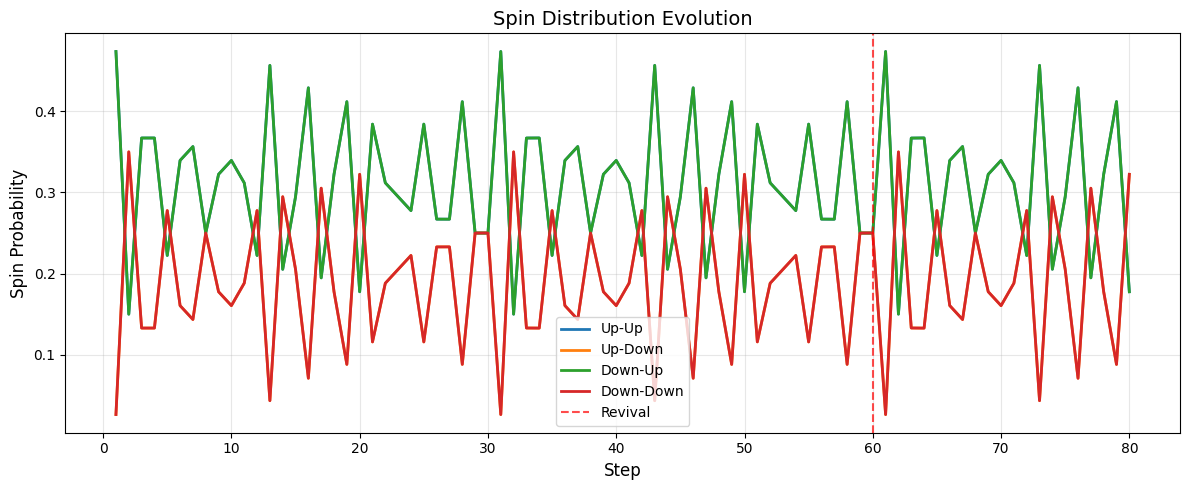
\includegraphics[width=0.95\linewidth]{fig-10x10-spin.png}
  \caption{Spin (coin) distribution over eighty steps for the
           $10 \times 10$ torus at $\rho = (5-\sqrt{5})/10$,
           $\delta = 0$. The four coin components return to their
           initial values at both $N = 30$ and $N = 60$. The return at
           $N = 30$ is a partial revival of the coin alone; only at
           $N = 60$ does the position distribution also coincide with
           the initial condition, producing the full-state revival.}
  \label{fig:10x10-spin}
\end{figure}
